\documentclass[12pt, a4paper]{article}

% Packages
\usepackage{enumerate}
\usepackage{amsmath, amsfonts, amssymb}
\usepackage{geometry}
\usepackage{graphicx}
\usepackage{pgfplots}
\usepackage{caption}
\usepackage{subcaption}
\usepackage[colorlinks=true,linkcolor=cyan]{hyperref}

\pgfplotsset{compat=1.18}

% Configurations
\geometry{left=1in, right=1in, top=0.5in, bottom=0.5in}  % margins
\numberwithin{equation}{section} % equation numbering

% New Commands
\newcommand{\primed}[1]{#1^{\prime}}
\newcommand{\tp}{\primed{t}}	% t prime
\newcommand{\omegap}{\primed{\omega}}	% omega prime
\newcommand{\xip}{\primed{\xi}}	% xi prime

\newcommand{\diff}{\mathop{}\!\mathrm{d}}
\newcommand{\dx}{\diff x}
\newcommand{\dy}{\diff y}
\newcommand{\dt}{\diff t}
\newcommand{\dtp}{\diff \tp}
\newcommand{\domega}{\diff \omega}
\newcommand{\domegap}{\diff \omegap}
\newcommand{\dxi}{\diff \xi}
\newcommand{\dxip}{\diff \xip}
\newcommand{\derv}[1]{\frac{\diff \hfill}{\diff #1}}	% Derivative without brackets
\newcommand{\dervb}[2]{\derv{#1} \left(#2\right)}  % Derivative with brackets
\newcommand{\dervsb}[2]{\derv{#1} \left[#2\right]}  % Derivative with square brackets

\newcommand{\pdiff}{\mathop{}\!\mathrm{\partial}} % Partial Differential sign
\newcommand{\pdx}{\pdiff x}
\newcommand{\pdy}{\pdiff y}
\newcommand{\pdt}{\pdiff t}
\newcommand{\pdtp}{\pdiff \tp}
\newcommand{\pdomega}{\pdiff \omega}
\newcommand{\pdomegap}{\pdiff \omegap}
\newcommand{\pdxi}{\pdiff \xi}
\newcommand{\pdxip}{\pdiff \xip}

\newcommand{\pderv}[1]{\frac{\pdiff \hfill}{\pdiff #1}}	% Partial Derivative without brackets
\newcommand{\pdervb}[2]{\pderv{#1} \left(#2\right)}  %Partial Derivative with brackets
\newcommand{\pdervsb}[2]{\pderv{#1} \left[#2\right]}  % Partial Derivative with square brackets

\newcommand{\dint}[2]{\int \limits_{#1}^{#2}}  % definite integral
\newcommand{\intinfty}{\dint{-\infty}{\infty}}	% Integral from -infty to infty
\newcommand{\intzerotoinfty}{\dint{0}{\infty}}	% integral from 0 to infty

% Global Info
\title{Fourier Transform: An intuitive approach}
\author{Rohan Singh Chauhan}
\date{February 4, 2023}

% Main Document
\begin{document}
\maketitle

\begin{figure}
	\centering
	\subfloat[$k = 10$] {
		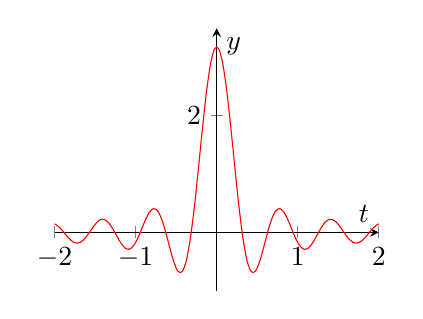
\begin{tikzpicture}
			\begin{axis} [
					axis lines=middle, 
					xmin=-2, 
					xmax=2, 
					ymin=-1,
					ymax=3.5,
					xlabel=$t$, 
					ylabel=$y$, 
					ylabel style={rotate=0}, 
					width=0.47\linewidth
				]
				
				\addplot[
				smooth,
				color=red, 
				samples=200,
				mark=false
				] {
					sin(deg(10 * x)) / (pi * x)
				};
				
			\end{axis}
		\end{tikzpicture}
	}\hfill
	\subfloat[$k = 1000$] {
		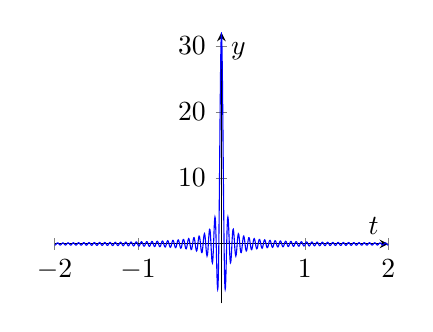
\begin{tikzpicture}
%			\begin{axis} [     % k=50
%				axis lines=middle, 
%				xmin=-2, 
%				xmax=2, 
%				ymin=-3,
%				ymax=16,
%				xlabel=$t$, 
%				ylabel=$y$, 
%				ylabel style={rotate=0}, 
%				width=0.45\linewidth
%				]
%				
%				\addplot[
%				smooth,
%				color=blue, 
%				samples=200,
%				mark=false
%				] {
%					sin(deg(50 * x)) / (pi * x)
%				};
%				
%			\end{axis}
			\begin{axis} [
				axis lines=middle, 
				xmin=-2, 
				xmax=2, 
				ymin=-9,
				ymax=32,
				xlabel=$t$, 
				ylabel=$y$, 
				ylabel style={rotate=0}, 
				width=0.48\linewidth
				]
				
				\addplot[
				smooth,
				color=blue, 
				samples=2000,
				mark=false
				] {
					sin(deg(100 * x)) / (pi * x)
				};
				
			\end{axis}
		\end{tikzpicture}
	}

	\caption{Plot of $\sin(kt)/\pi t$ against $t$ for different $k > 0, k \in \mathbb{R}$. As $k$ increases, function approaches $k/\pi$ for $t = 0$ and tends to $0$ for $t \neq 0$}
\end{figure}

\end{document}